Establece que el ángulo de incidencia de un rayo en una superficie es igual al ángulo de reflexión, ambos medidos con respecto a la normal de la superficie.

\begin{figure}[H]
  \centering
  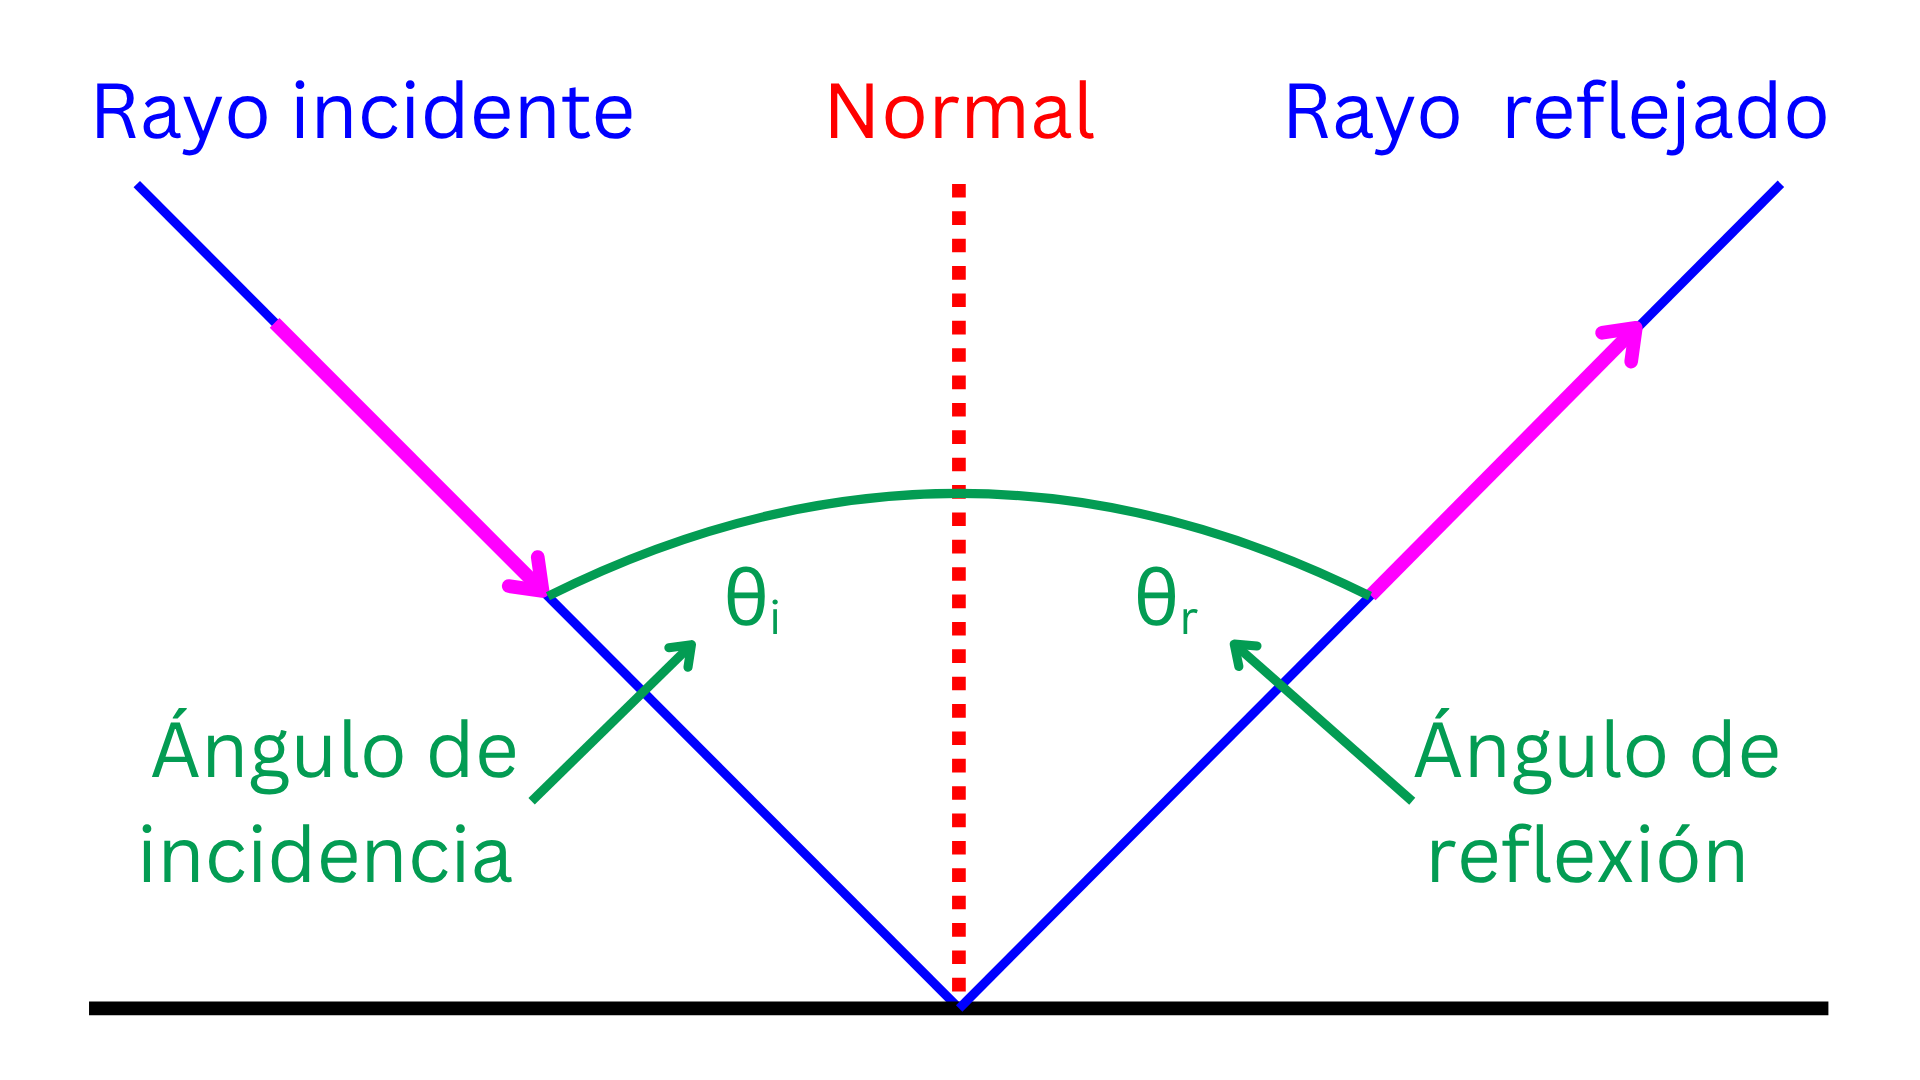
\includegraphics[scale=0.2]{imagenes/ley_reflexion.png}
  \caption{Ley de reflexión}
\end{figure}

Elementos:

\begin{itemize}
  \item \textbf{Rayo incidente:} Onda que entra o impacta con la superficie.
  \item \textbf{Rayo reflejado:} Onda que sale o rebota de la superficie.
  \item \textbf{Normal:} Linea imaginaria perpendicular a la superficie en el punto donde el rayo incide.
  \item \textbf{Ángulo de incidencia $(\theta_i)$:} Ángulo formado entre el rayo incidente y la normal.
  \item \textbf{Ángulo de reflexión $(\theta_r)$:} Ángulo formado entre el rayo reflejado y la normal.
\end{itemize}

Considerando un ángulo de incidencia $\theta_i$ y un ángulo de reflexión $\theta_r$, la ley se expresa de la siguiente forma:

\begin{listequbox}
  {\theta_i = \theta_r}{equleyrfl}{Ley de reflexión}
\end{listequbox}
